\documentclass[tikz, border=1mm]{standalone}
\usepackage{tikz}
\usepackage{graphicx}
\definecolor{grey}{rgb}{0.8,0.8,0.8}
\definecolor{grey2}{rgb}{0.5,0.5,0.5}
\usetikzlibrary{positioning}
\usetikzlibrary{quotes}
\begin{document}
\begin{tikzpicture}[
squarednodepsi2/.style={rectangle, draw=red!60, fill=red!5,text width=10em, text height=4em, align=center,very thick, minimum size=7mm, rounded corners},
squarednodepsi/.style={rectangle, draw=red!60, fill=red!5,text width=7em, align=center,very thick, minimum size=7mm, rounded corners},
squarednode/.style={rectangle, draw=blue!60, fill=blue!5,text width=10em, align=center,very thick, minimum size=5mm, rounded corners},
squarednode2/.style={rectangle, draw=black!60, fill=grey2!5,text width=10em, align=center,very thick, minimum size=5mm, rounded corners},
squarednode3/.style={rectangle, draw=blue!60, fill=blue!5,text width=12em, align=center,very thick, minimum size=5mm, rounded corners},
squarednodethin/.style={rectangle, draw=blue!60, fill=blue!5,text width=5em, align=center,very thick, minimum size=5mm, rounded corners},
]
%Nodes
\node[squarednode]      (maintopic)                              {3.) Train $n_{\mathrm{RBM}}$ RBMs.};
\node[squarednode2] at (0,2)       (reference)       {2.) Choose a \textit{reference} measurement configuration.};
\node[squarednode2] at (0,3.5)        (firstmeasure)      {1.) Measure a few samples.};
\node[squarednodepsi2] at (0,5.6)       (psitarget)        {target state $\psi_{\mathrm{target}}$};
%\node[inner sep=0pt] (psitargetfigure) at (0,1){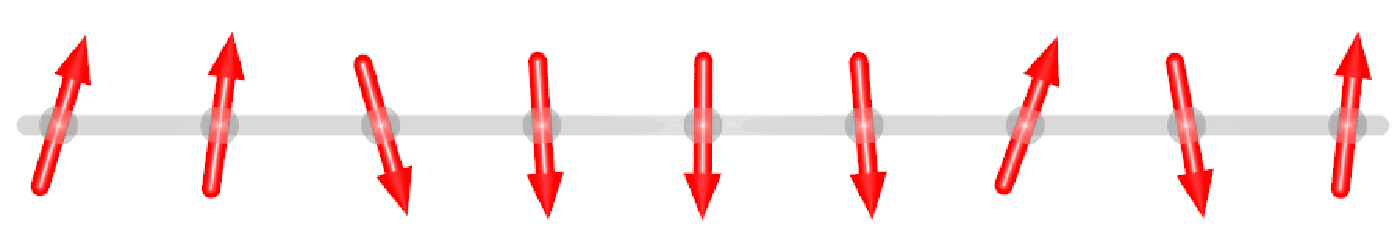
\includegraphics[width=.25\textwidth]{targetstate.pdf}}

\node[squarednodepsi]      (psiRBM)       [right=of maintopic] {reconstructed state $\psi_{\mathrm{AL}}$};
\node[squarednode3]        (commitee)       [below=of maintopic] {4.) \textit{Query-by-Commitee}: Decide which measurement configuration is most informative.};
\node[squarednodethin]        (measure)       [left=of maintopic, yshift=-1cm, xshift=-0.5cm] {Measure in requested configuration.};




%Lines
\draw[line width=0.7mm, ->, color=grey] (psitarget.south) -- (firstmeasure.north);
\draw[line width=0.7mm, ->, color=grey] (firstmeasure.south) -- (reference.north);
\draw[->, line width=0.7mm, color=grey] (reference.south) -- (maintopic.north);
\draw[->, line width=0.7mm, color=grey] (maintopic.south) -- (commitee.north);
\draw[->, line width=0.7mm, color=grey] (measure.east) -- (maintopic.west);
\draw[->, line width=0.7mm, color=grey] (maintopic.east) -- (psiRBM.west);
\draw[->, line width=0.7mm, color=grey] (commitee.west) --(measure.east);

\draw[->, line width=0.7mm, color=grey] (0.5,-0.5) --(0.5,-1.5);
\draw[->, line width=0.7mm, color=grey] (-0.5,-0.5) --(-0.5,-1.5);
\draw[->, line width=0.7mm, color=grey] (1,-0.5) --(1,-1.5);
\draw[->, line width=0.7mm, color=grey] (-1,-0.5) --(-1,-1.5);
\draw[->, line width=0.7mm, color=grey] (1.5,-0.5) --(1.5,-1.5);
\draw[->, line width=0.7mm, color=grey] (-1.5,-0.5) --(-1.5,-1.5);

\node at (0,5.8){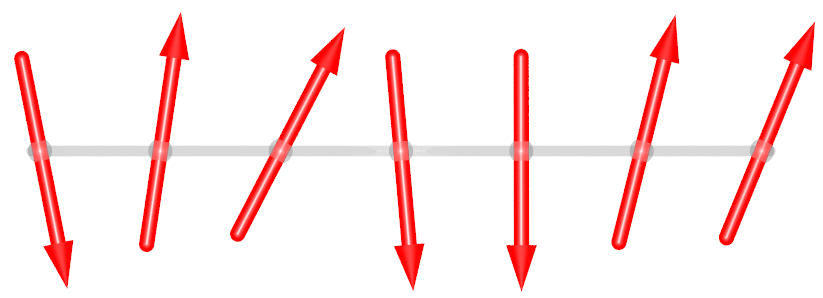
\includegraphics[width=3cm]{targetstate.png}} ;

\end{tikzpicture}
\end{document}

